\chapter{Design}
\label{cap:design}

\section{Class Diagram}
\label{sec:class_diagram}

\subsection{VOPC (Analysis)}
\label{subsec:vopc}

\begin{figure}[H]
    \centering
    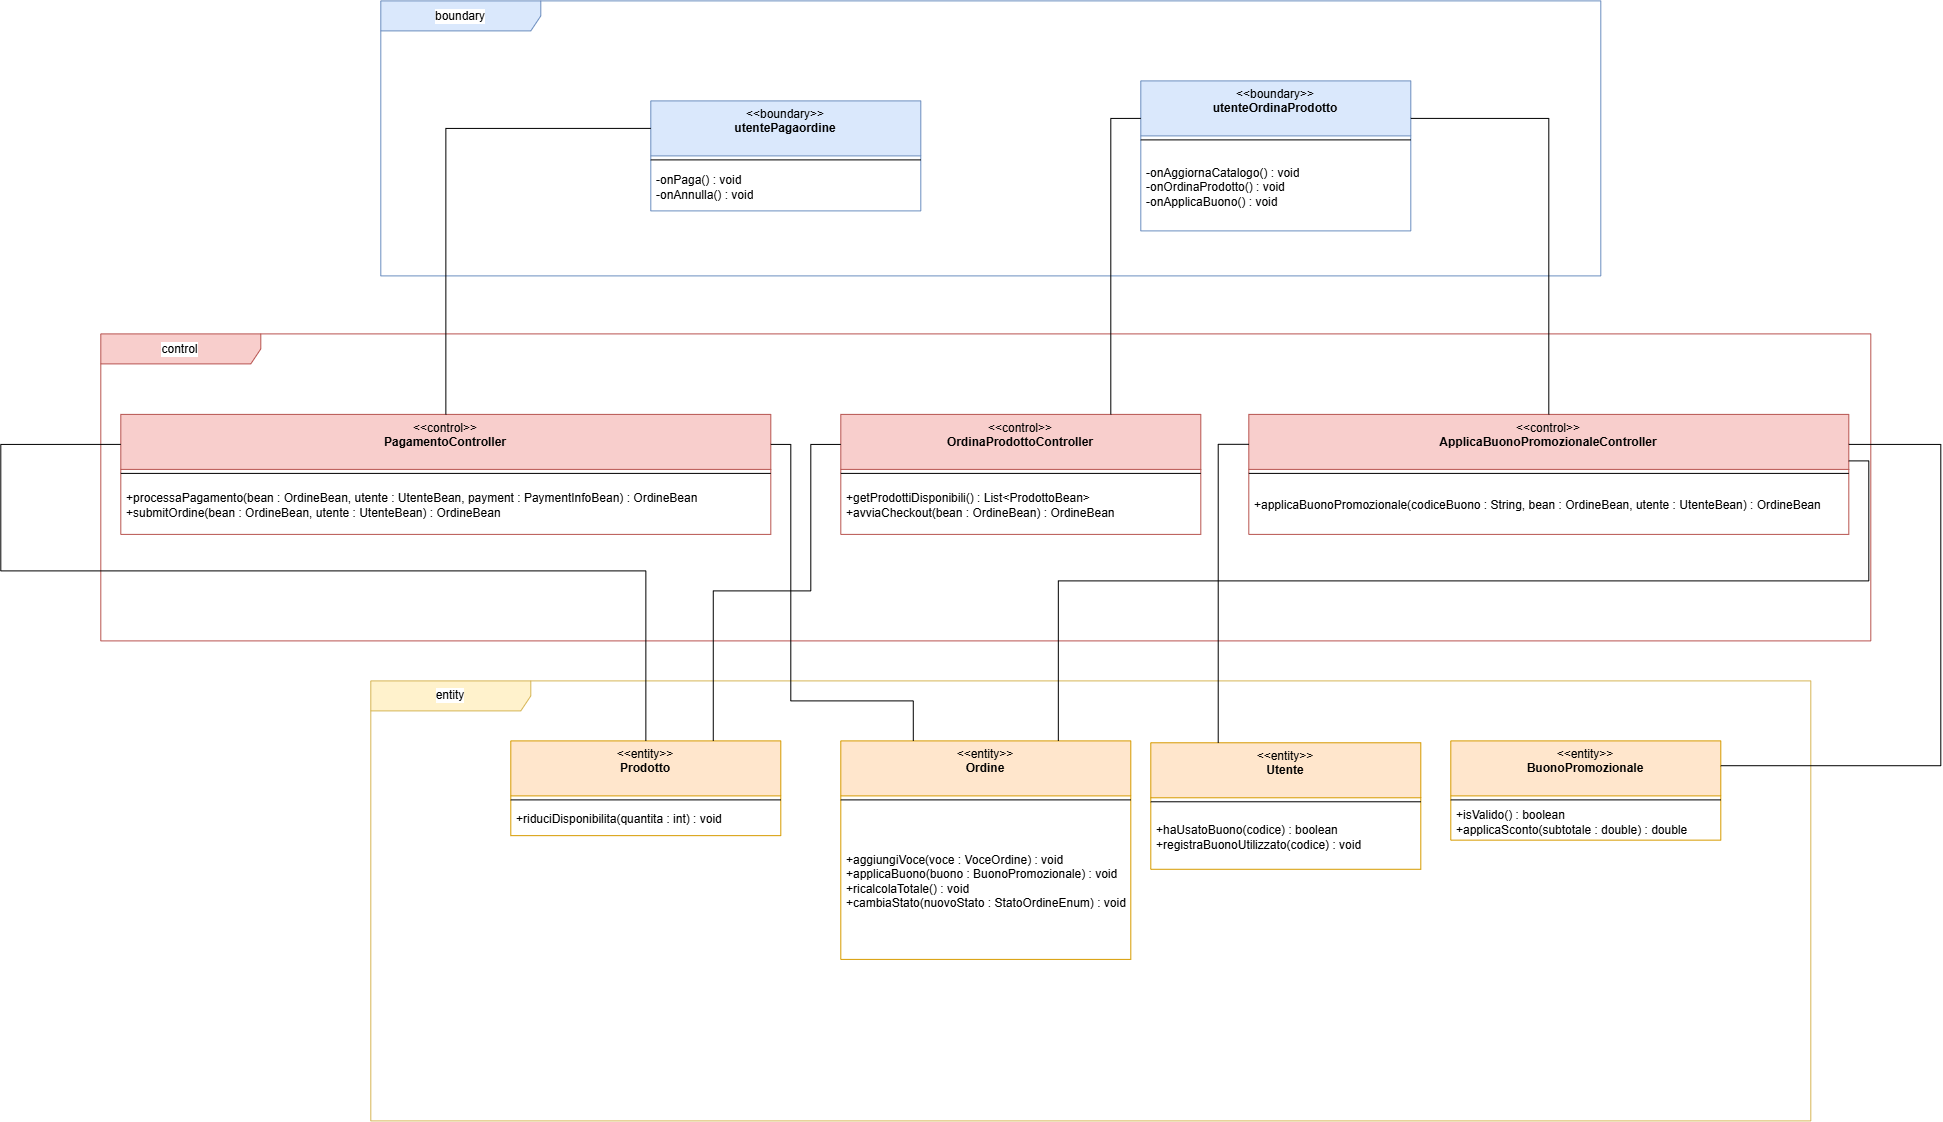
\includegraphics[width=\textwidth]{figures/vopc_uc04.png}
    \caption{VOPC of UC-04: Boundary (View), graphic controller, Facade, application controllers and Entity.}
    \label{fig:vopc}
\end{figure}

\subsection{Design Patterns}
\label{subsec:design_patterns}
The design level introduces the interfaces, the Java types, the exceptions and
the GoF patterns to manage extensibility and dynamic persistence (NFR-01). For
each pattern, the schema and a short description of its application are shown
in order.

\subsubsection*{Abstract Factory Pattern -- Persistence Layer}
\begin{figure}[H]
    \centering
    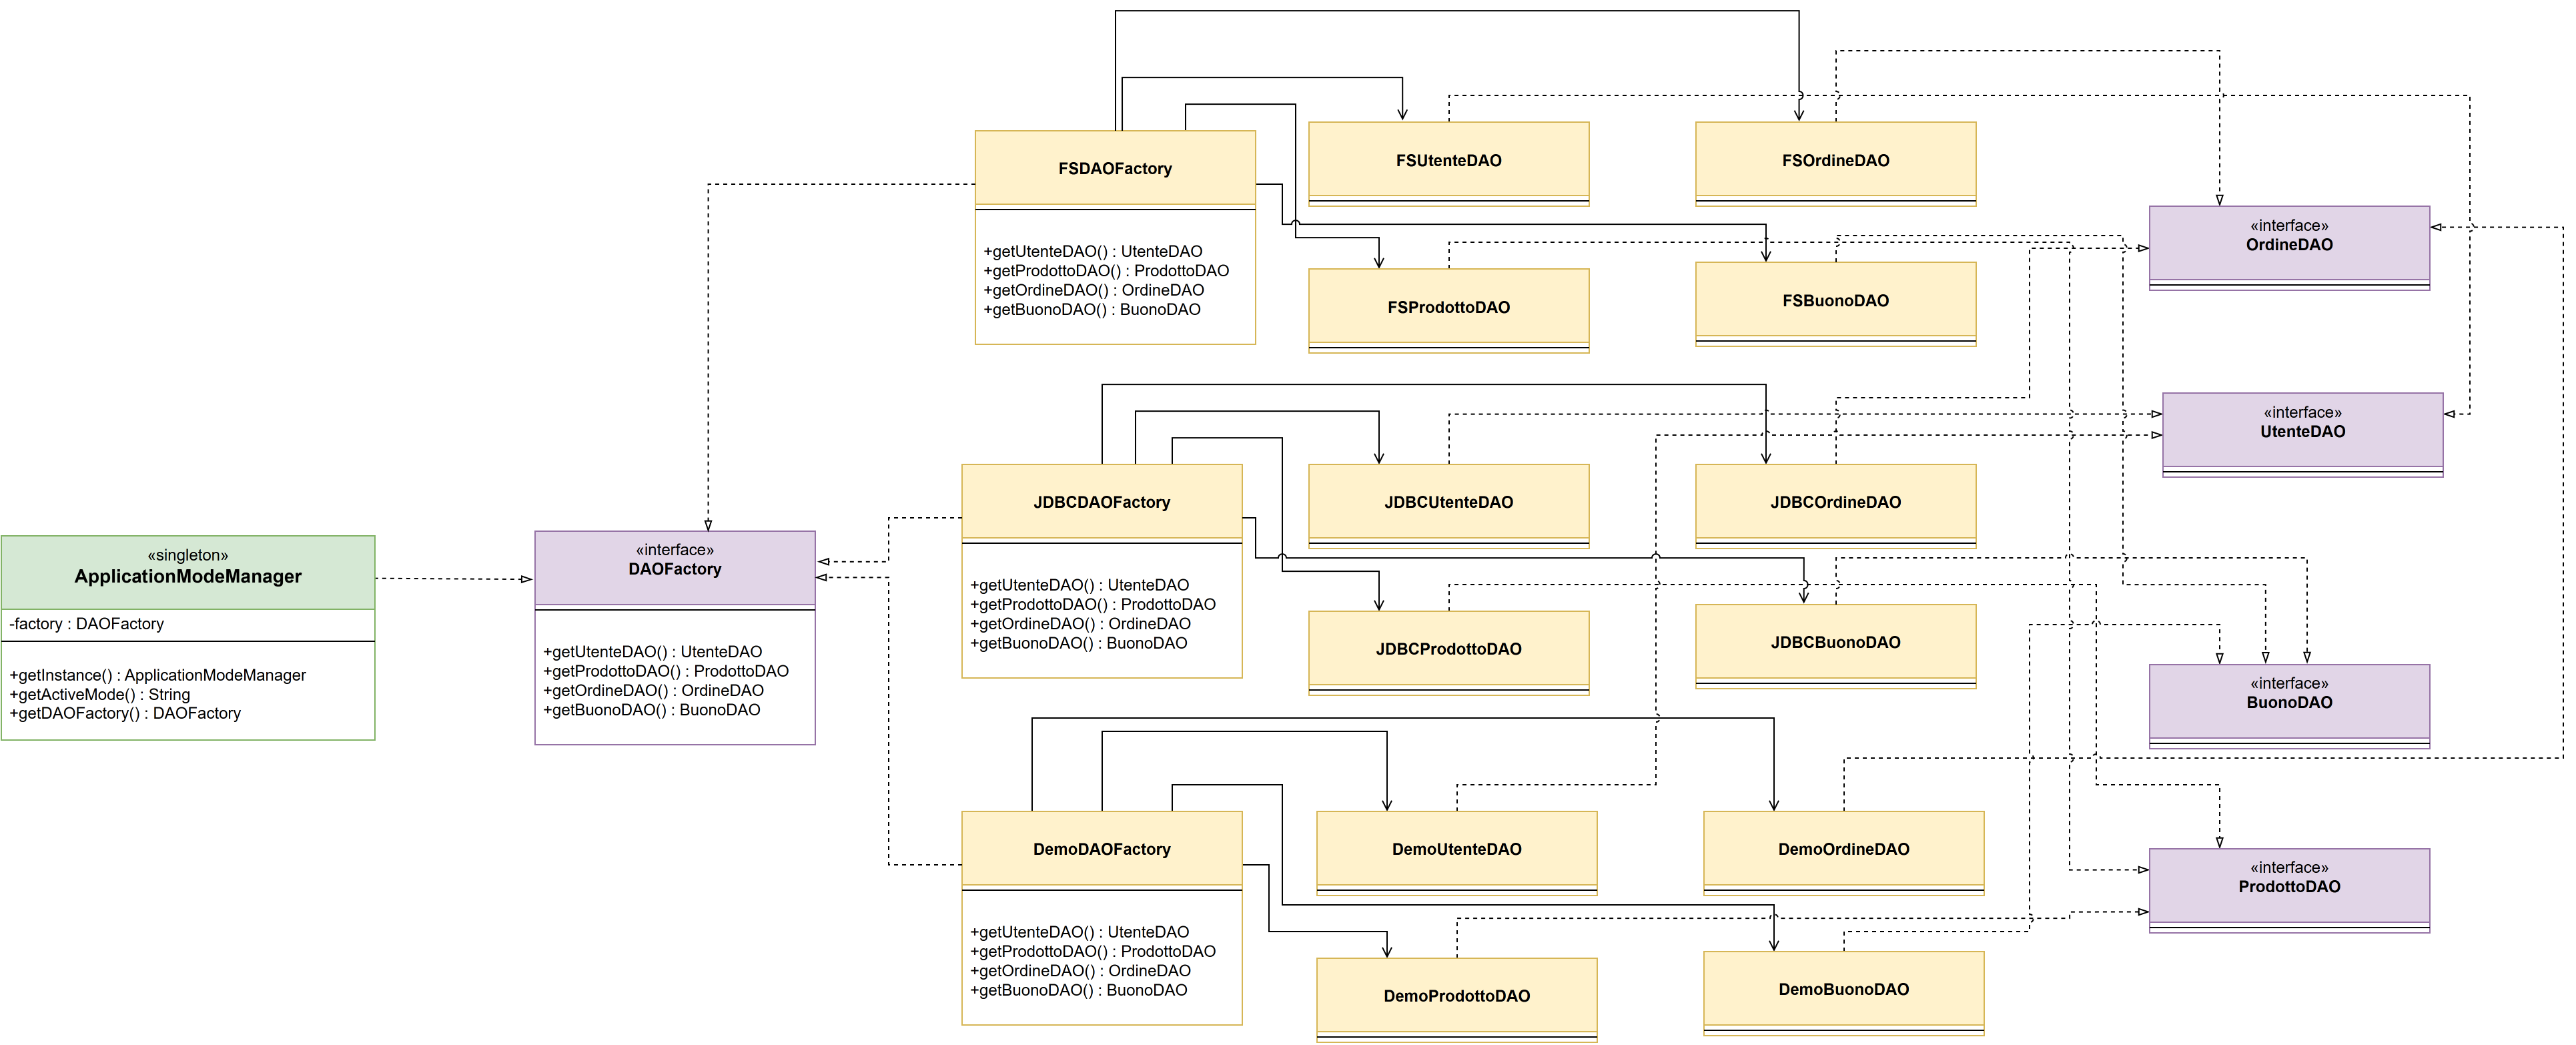
\includegraphics[width=0.85\textwidth]{figures/dl_factory_hr.png}
    \caption{Abstract Factory of the persistence: DAO interfaces, concrete DAOs and factories.}
    \label{fig:dl_factory}
\end{figure}
The persistence layer is managed through the \textbf{Abstract Factory} pattern
in order to guarantee flexibility in configuring the execution environment. The
\texttt{DAOFactory} interface defines the contract for creating the different
Data Access Objects, such as \texttt{getOrdineDAO()} and \texttt{getProdottoDAO()}.
According to the \texttt{persistence\_type} property, the concrete factories
(\texttt{JDBCDAOFactory}, \texttt{FSDAOFactory}, \texttt{DemoDAOFactory})
instantiate the appropriate storage implementation. This allows the system to
switch seamlessly between a database-based, file-system-based or in-memory
persistence without requiring any change in the client code.

\subsubsection*{Observer Pattern -- Notification System}
\begin{figure}[H]
    \centering
    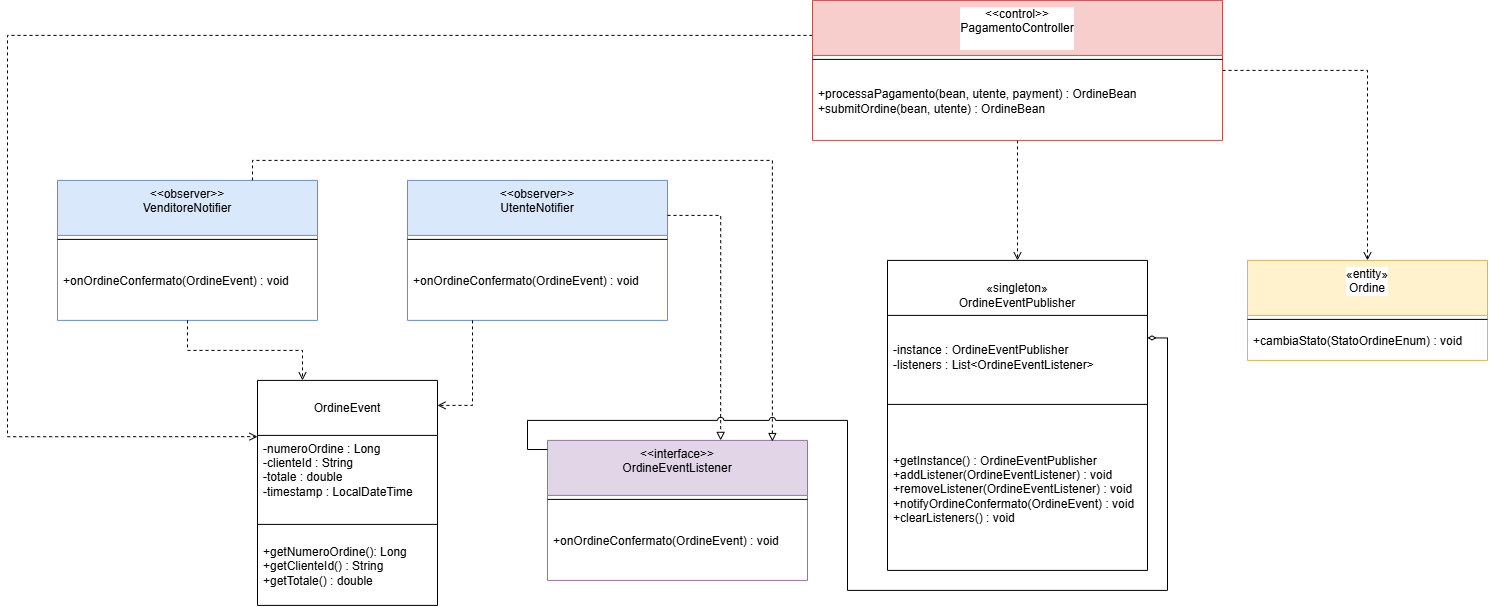
\includegraphics[width=0.55\textwidth]{figures/dl_observer_hr.png}
    \caption{Observer of the order confirmation: singleton publisher and DTO.}
    \label{fig:dl_observer}
\end{figure}
The \textbf{Observer} pattern has been implemented with the aim of decoupling
the order processing from the notification management logic. The
\texttt{OrdineEventPublisher} class acts as a \emph{Subject} implemented through
the \textbf{Singleton} pattern, managing a list (\texttt{List}) of observers of
type \texttt{OrdineEventListener}. Upon the correct submission and confirmation
of the order, the publisher invokes the \texttt{onOrdineConfermato()} method on
all the registered listeners (buyer and vendor), passing the read-only DTO
\texttt{OrdineEvent}, never the domain entity. This architecture guarantees
loose coupling between the main business logic and its side effects, strictly
respecting the \emph{Open/Closed Principle}.

The notification is emitted by the application subsystem (the control that
confirms the order) through the publisher, and not by the \texttt{Ordine}
entity: the domain entity thus remains \emph{decoupled} from the presentation
layer and from the notification mechanism. The variant is the
\emph{publish-subscribe}/event-driven one of the Observer: the coupling between
\texttt{OrdineEventPublisher} (Subject) and the observers is abstract (only
\texttt{OrdineEventListener}), the notification is a broadcast to all the
registered listeners and the exchanged data is the read-only DTO
\texttt{OrdineEvent}, never the entity.

\subsubsection*{Singleton Pattern -- Sessions and Mode}
\begin{figure}[H]
    \centering
    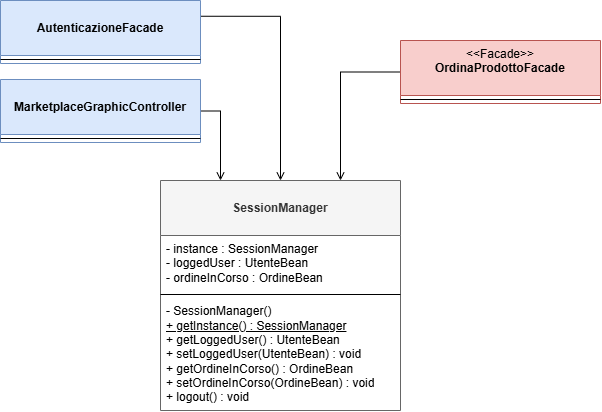
\includegraphics[width=0.55\textwidth]{figures/dl_singleton_hr.png}
    \caption{Singleton of the session and of the mode.}
    \label{fig:dl_singleton}
\end{figure}
\texttt{SessionManager} (user session) and \texttt{ApplicationModeManager}
(application mode) adopt a classic singleton with \emph{lazy
initialization} (\texttt{if (instance == null) instance = new X()}) and
synchronization on \texttt{getInstance()}, in line with the reference projects:
no perceivable cost in a desktop client, no SonarCloud warning suppression.

\subsubsection*{Facade Pattern -- Checkout UC-04}
\begin{figure}[H]
    \centering
    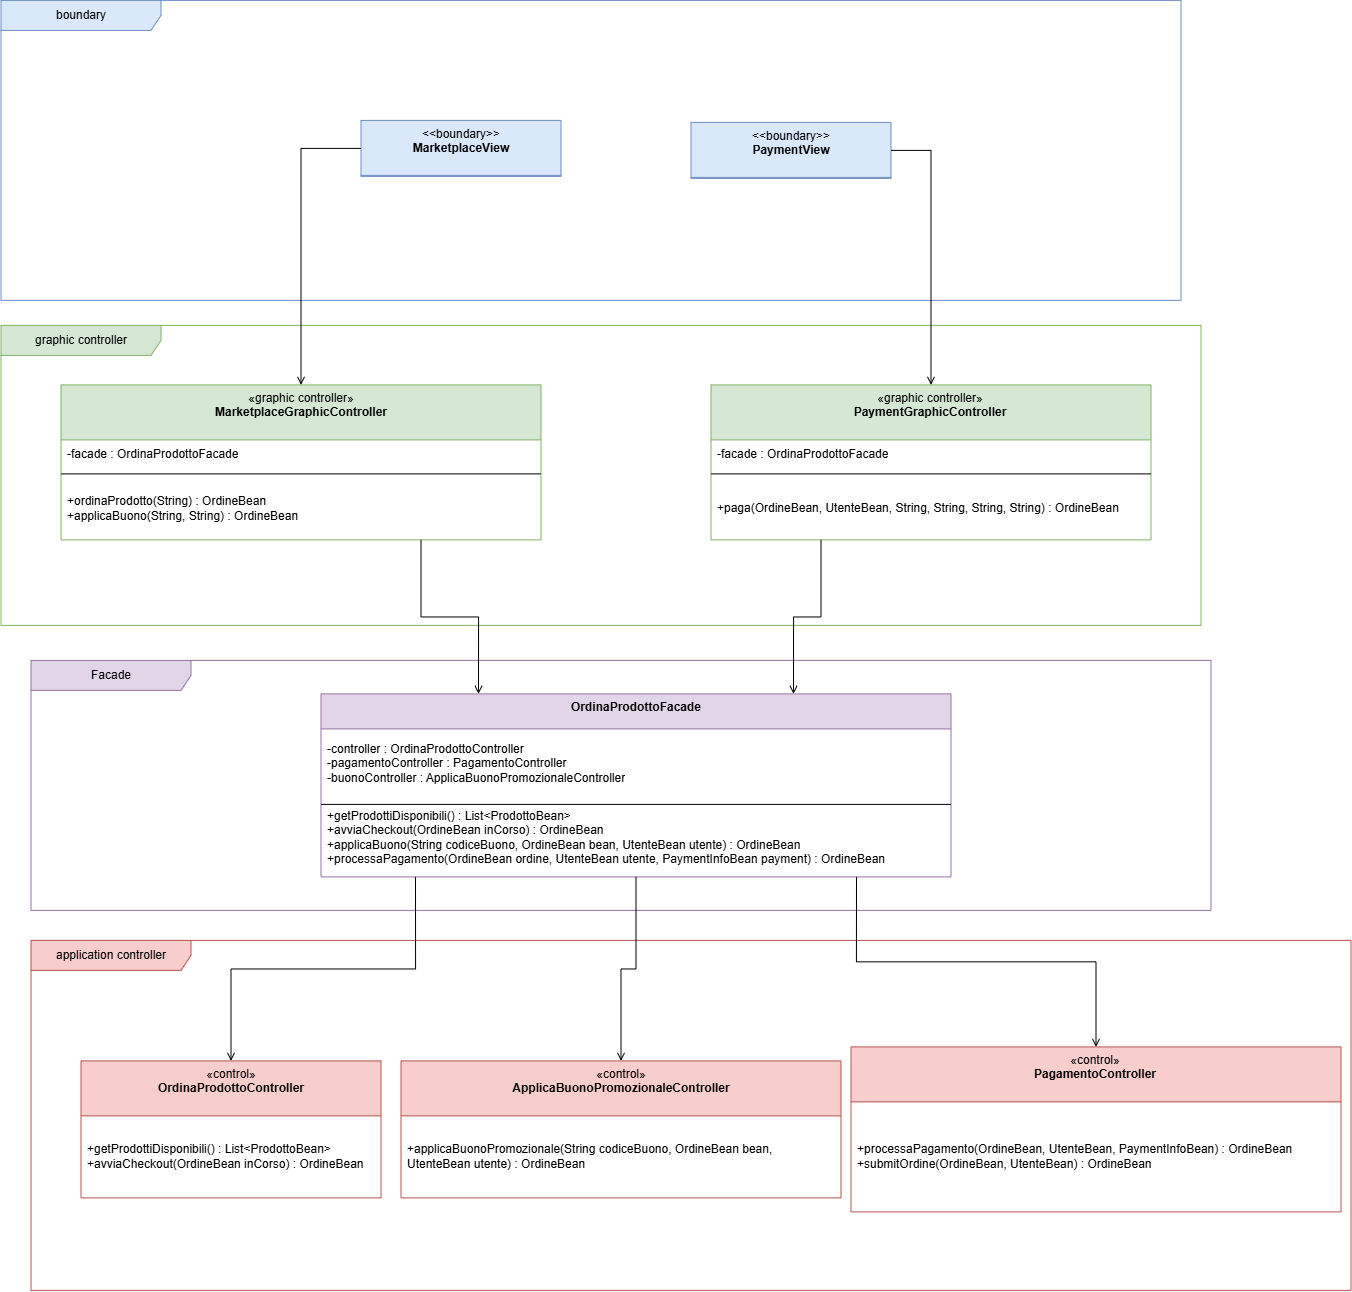
\includegraphics[width=0.75\textwidth]{figures/dl_facade_hr.png}
    \caption{Facade of the UC-04 checkout.}
    \label{fig:dl_facade}
\end{figure}
\texttt{OrdinaProdottoFacade} exposes to the graphic controller a single
interface for the checkout (\texttt{getProdottiDisponibili},
\texttt{avviaCheckout}, \texttt{applicaBuono}, \texttt{processaPagamento})
and hides the business subsystem, formed by the base controller and by the
extension controllers (voucher 4a and payment 6/6a). The client (boundary or
graphic controller) does not know the order in which the methods of the
application controllers are called. The operations of the extensions (
\texttt{applicaBuono}, \texttt{processaPagamento}) live only in their
respective sub-controllers: the Facade invokes them directly and the base
controller does not re-expose them (no useless pass-through / indirection).

\section{Activity Diagram}
\label{sec:comportamentale}

\begin{figure}[H]
    \centering
    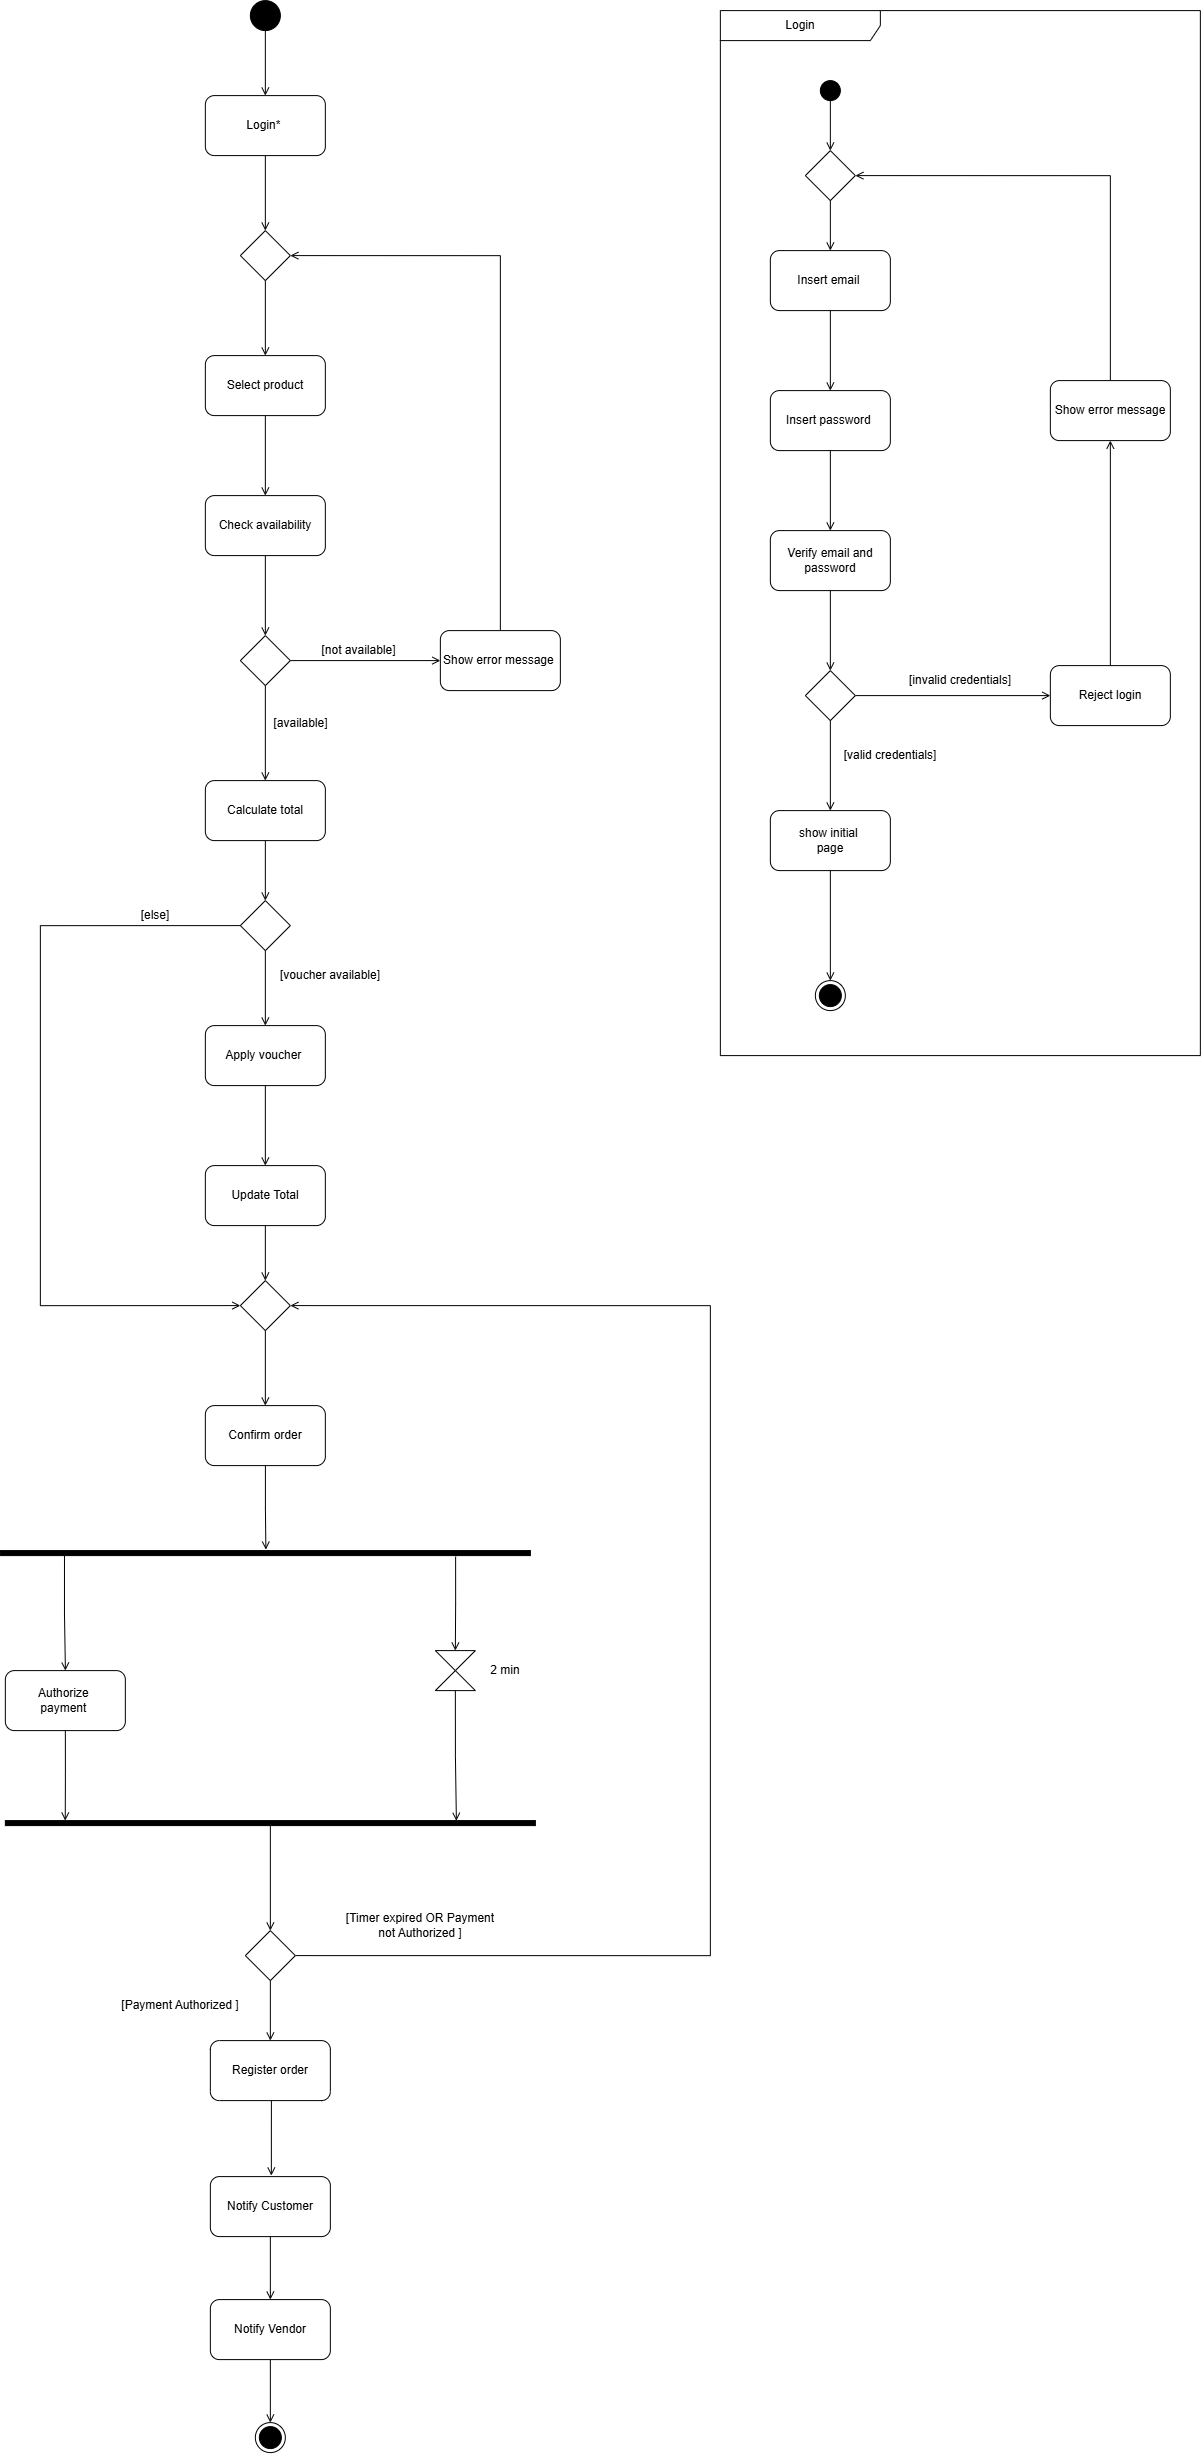
\includegraphics[height=0.8\textheight]{figures/activity_uc04.png}
    \caption{Activity diagram of UC-04: availability check, voucher application,
    payment authorization and sequential notification to buyer and vendor.}
    \label{fig:activity}
\end{figure}

\section{Sequence Diagram}
\label{sec:sequence}

\begin{figure}[H]
    \centering
    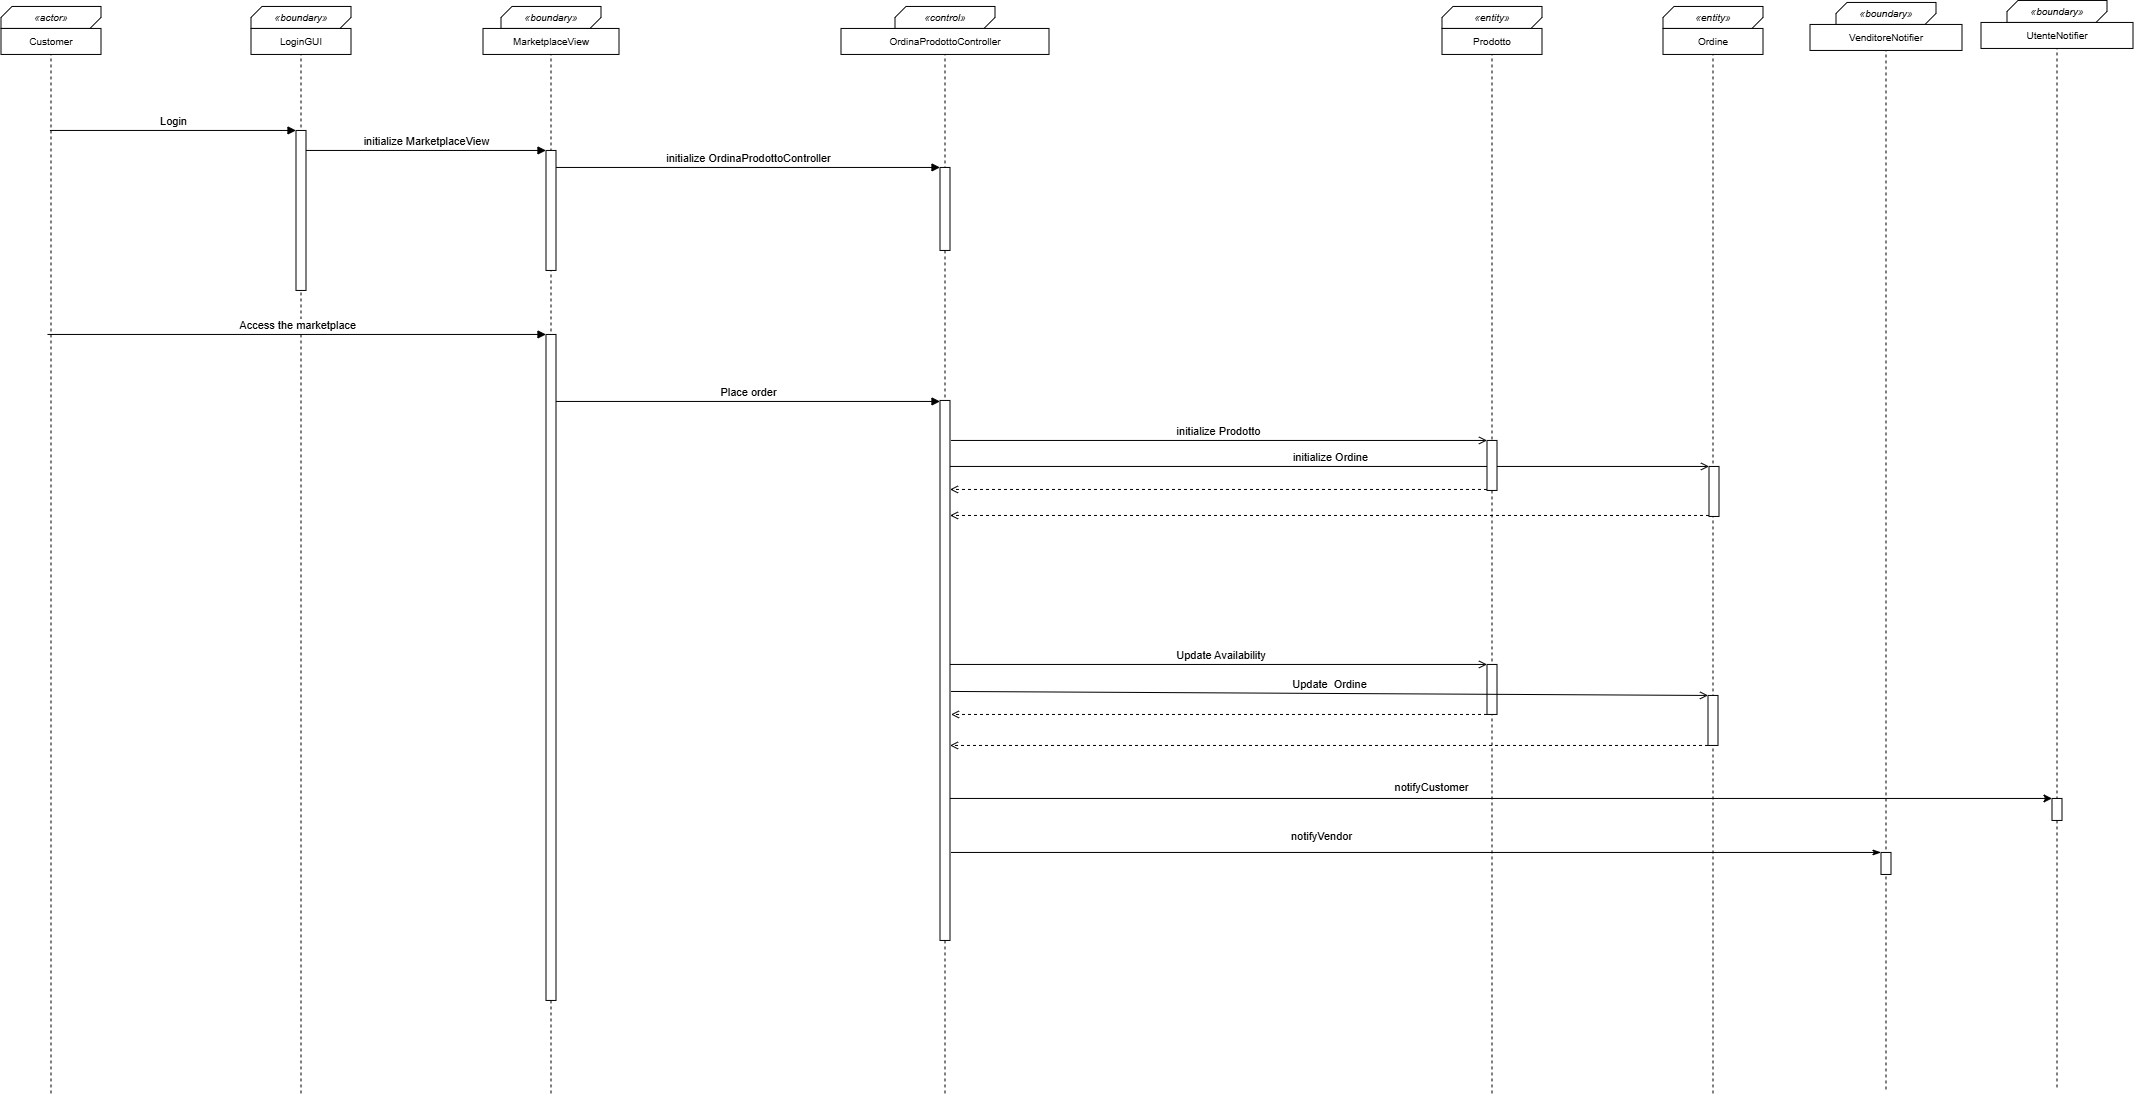
\includegraphics[width=\textwidth]{figures/seq_uc04_clean.png}
    \caption{Sequence diagram of UC-04.}
    \label{fig:sequence}
\end{figure}

\section{State Diagram}
\label{sec:state}

\begin{figure}[H]
    \centering
    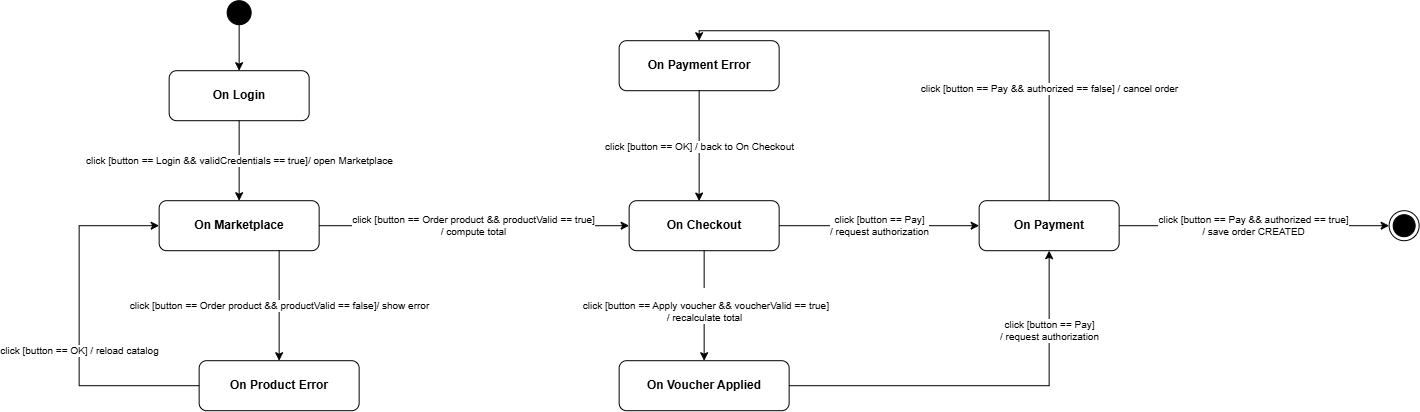
\includegraphics[width=\textwidth]{figures/state_uc04.png}
    \caption{State diagram of UC-04 Order a Product: navigation and alternative flows \texttt{3a}, \texttt{4a} and \texttt{6a}.}
    \label{fig:state}
\end{figure}

